%!TEX root =  concept_mining.tex


\begin{table*}
\small
\centering
\begin{tabular}{llllll} 
\toprule
Datasets & Task & Domain & Metric & $\vert$ Train$\vert$ & $\vert$Test$\vert$  \\
\midrule

Sample Text & \multirow{5}{*}{\begin{tabular}[c]{@{}l@{}}Text Modeling\end{tabular}}  & General text           & \multirow{5}{*}{\begin{tabular}[c]{@{}l@{}}Word prediction + \\ Next sentence prediction\end{tabular}} & 16   & 480     \\
Sample Large &                         & General text &       & 280K  & 8.4M     \\
Wikitext-2 converted       &                         & Articles from Wikipedia &   & 60K  & 1800K     \\
Arxiv Computer Science      &                         & Technical papers from \url{arxiv.org}  &       & 362K  & 1.1M     \\
Arxiv Math       &                         & Technical papers from \url{arxiv.org} &      & 175K  & 525K     \\
\midrule
CoLA & classification  & Books and journal articles  & Matthews coefficient      & 8.5k & 1k    \\
\midrule
MRPC &  \multirow{2}{*}{\begin{tabular}[c]{@{}l@{}}paraphrase\end{tabular}}  & News &  \multirow{2}{*}{\begin{tabular}[c]{@{}l@{}}Accuracy / F1\end{tabular}} 
& 3.7k & 1.7k   \\
QQP &                         & Questions from Quora &      & 364k & 391k  \\ 
\midrule
STS-B & Sentence Similarity                    & Misc.    & Pearson/Spearman       & 7k & 1.4k  \\
\midrule
MNLI        &  \multirow{2}{*}{\begin{tabular}[c]{@{}l@{}}NLI\end{tabular}}                   & Internet Crawl  & \multirow{2}{*}{\begin{tabular}[c]{@{}l@{}}Accuracy\end{tabular}}      &393k & 20k   \\
RTE      &          & Wikipedia             &      &  2.5k & 3k  \\
\midrule
QNLI     & QA + NLI & News and Wikipedia   & \multirow{2}{*}{\begin{tabular}[c]{@{}l@{}}Accuracy\end{tabular}}      & 105k & 5.4k  \\
WNLI        & coreference + NLI & Fiction books   &        & 634 & 146  \\
\bottomrule
\end{tabular}
\caption{An overview of the benchmark datasets used for different tasks along with their description and statistics}
\label{tab:dataset}
\end{table*}





\begin{figure*}
\begin{minipage}[b]{.5\linewidth}
 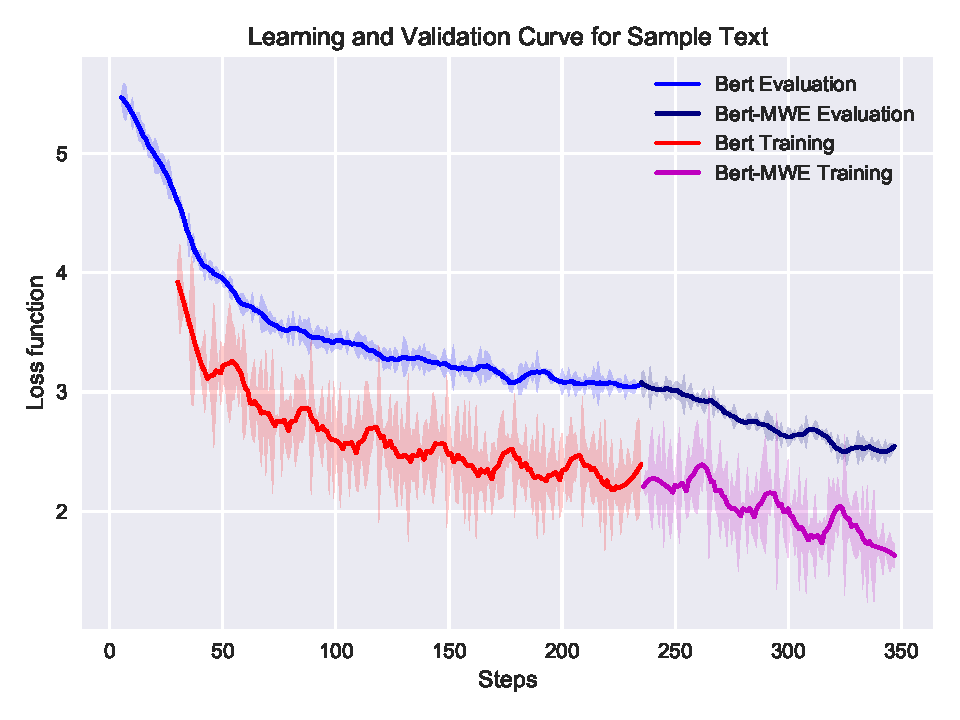
\includegraphics[width=\linewidth]{fig/st.pdf}
\label{fig:manual-eval1}
\end{minipage}
\begin{minipage}[b]{.5\linewidth}
 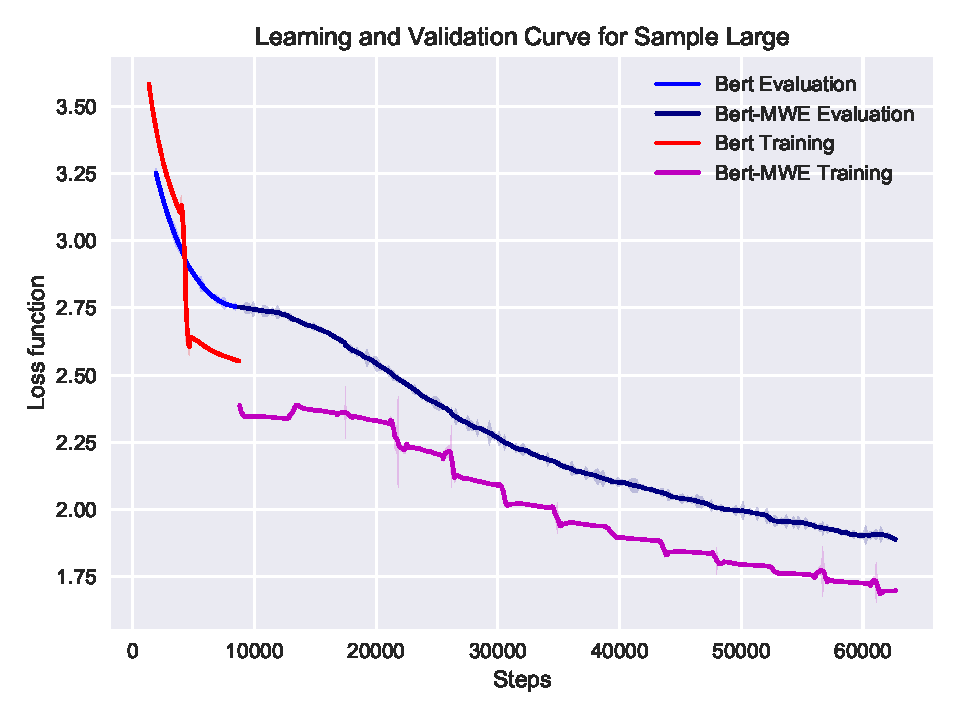
\includegraphics[width=\linewidth]{fig/sl.pdf}
\label{fig:manual-eval2}
\end{minipage}
\vspace{-15pt}
\caption{Learning and validation curve for the text modeling task}
\label{fig:learning-curve}
%\vspace{3pt}
\end{figure*}





\begin{table*}
\begin{center}
\begin{tabular}{lllclcllc} 
\toprule
System      & CoLA                                                                         & MRPC                                                                              & QQP                           & STS-B              & QNLI                     & MNLI          & RTE           & WNLI                      \\ 
\hline
BiLSTM      & 11.6                                                                         & 81.8/74.3                                                                         & \multicolumn{1}{l}{62.5/84.2} & 70.3/67.8          & \multicolumn{1}{l}{74.6} & 65.6          & 57.4          & \multicolumn{1}{l}{65.1}  \\
BiLSTM+Attn & \textcolor[rgb]{0.133,0.133,0.133}{\textcolor[rgb]{0.133,0.133,0.133}{18.6}} & \textcolor[rgb]{0.133,0.133,0.133}{\textcolor[rgb]{0.133,0.133,0.133}{83.9/76.2}} & 72.8/70.5                     & 72.8/709           & 74.3                     & 67.6          & 58.4~ ~~      & 65.1                      \\
OpenAI GPT  & 45.4                                                                         & 82.3/-                                                                            & 70.3/-                        & 80.0/-             & 87.4                     & 82.1          & 56.0          & 65.1                      \\
Bert        & 57.9                                                                         & 86.0/89.9                                                                         & 89.9/86.7                     & 89.6/89.2          & 90.8                     & 83.4          & 67.1          & 57.7                      \\
\BertMWE (Simplified)     & 58.1                                                                         & 86.0/89.9                                                                         & 90.7/87.5                     & \textbf{90.0}/89.5 & 91.3                     & \textbf{84.0} & \textbf{72.2} & 56.3                      \\
    \BertMWE        & \textbf{59.7}                                                                & \textbf{86.5/90.4~}                                                               & \textbf{90.9/87.7}            & \textbf{90.0/89.6} & \textbf{91.5}            & \textbf{84.0} & \textbf{72.2} & \textbf{63.4}             \\
\bottomrule
\end{tabular}

   \caption{Performance on supervised label prediction}
   \label{tab:glue_results}
\end{center}
\end{table*}



\section{Experiments}\label{sec:bert_mwe_experiments}

In this section we experimentally evaluate the proposed approach over an wide range of tasks across different domains and demonstrate its effectiveness over the state of the art baseline approaches.




\subsection{Setup}

\noindent \textbf{Hardware Environment}
The model training and prepossessing is conducted on a lab server with 3 
GeForce RTX 2080 GPU card, 2 6-core Intel(R) Core(TM) i7-6800K CPU @ 3.40GHz CPU with 12GB memory. The longest experiments took no more than 3 days.


\noindent \textbf{Model architecture and hyper-parameter settings}
Since the proposed \BertMWE approach is built upon the Bert self-attention network architecture \cite{devlin2018bert},
and 
we're mainly interested in how much it can \textit{improve} upon the basic Bert model, 
we follow the exact same architecture, hyper-parameter and optimizer settings as suggested by 
\cite{devlin2018bert} for each specific tasks 
and refer the reader to the original paper for details about the architecture and parameter.

\noindent \textbf{Model training and weight initialization}
In order to more directly see the difference between the \BertMWE and the original Bert model, we conduct the model training of \BertMWE in an \textit{incremental} fashion:
we first follow the best training settings for each different variant of the Bert model  to train the basic model for a specific downstream task; after that, we start to train the corresponding \BertMWE 
for the Bert variant, and use the trained Bert model to initialize the \BertMWE. In other words, \BertMWE only changes the original Bert model with addition MWE structure, but retains all the trained weights.

\noindent \textbf{Model variants}
We apply the \BertMWE approach over the two different variants of Bert model as proposed in \cite{devlin2018bert}: the Bert-Finetune model where we use the pretrained weights as initialization, and fine-tune all layers of the model end to end; and the Bert-Feature model, where we freeze the pretrained  model weights and use the outputted hidden states as feature to train a task specific prediction head. 

We also 
explore two different variants of applying the non-compositionality.
The first is the theoretically sounded \BertMWE, which fully follows the variational inference procedure and learns a distribution over all possible models for prediction, as shown in \autoref{sec:var-param}; The second is a simplified version, 
 \BertMWE (Simplified), 
which do not add the \textit{MWE Dropout} layer to the network to explicitly utilize variational inference. 
However, it may still conduct inference over the importance of multi-word expressions to some extent by dynamically scale their inputted embedding to the downstream network.

\subsection{Text modeling} \label{sec:dataset}
We first evaluate the proposed approaches on on the task of modeling text data.
Specifically, we follow the construction of masked language model and next sentence prediction task \cite{devlin2018bert} to create our training and additionally a separate evaluation set, 
which shares no overlap with the training set. 
To make the competition fair with original Bert models, 
we will discard from the input text any MWEs that has overlaps with the masked position. 


We evaluate our approach over the following corpus. The dataset statistics are shown in \autoref{tab:dataset}. 


\begin{table*}[thbH]
\centering
\small
\begin{tabular}{lcccccc} 
\toprule
Datasets                                  & Training strategy                & Methods   & Evaluation~Loss ~ & Improvement            & ~Training Loss~        & Improvement              \\ 
\midrule
\multirow{6}{*}{Sample Text} & \multirow{2}{*}{Bert Finetune} & Base   & 0.39                & -                      & 0.001                     & -                        \\
                                               &                                & \BertMWE         & 0.290                & -25.7\%           & 0.000            & -66.7\%              \\
\cline{2-7}
                                               & \multirow{2}{*}{Bert Feature}  & Base  & 3.272                & -                      & 2.074                     & -                        \\
&                                & \BertMWE      & 2.35                & -28.2\%                      & 1.139                     & -45.1\%                       \\ 
\midrule
\midrule
\multirow{6}{*}{Sample Large} & \multirow{2}{*}{Bert Finetune} & Base   & 2.768                & -                      & 2.552                     & -                        \\
                                               &                                & \BertMWE      & 1.866                & -32.1\%                      & 1.670                     & - 34.56\%                       \\ 
\cline{2-7}
                                               & \multirow{1}{*}{Bert Feature}  & Base & 3.991                & -                      &         3.712            & -                        \\
                                               &                                & \BertMWE         & 3.918                 & -1.8\%           & 3.654            & -1.6\%              \\
\midrule
\midrule
\multirow{6}{*}{WikiText-2} & \multirow{2}{*}{Bert Finetune} & Base   & 1.851                & -                      & 0.588                                & -                        \\
&                                & \BertMWE      & 1.390                & -24.9\%                      & 0.489          & -16.8\%                       \\ 
\cline{2-7}
                                               & \multirow{2}{*}{Bert Feature}  & Base & 2.700                & -                      & 2.511                     & -                        \\
                                               &                                & \BertMWE         & 2.669                & -1.1\%           & 2.491            & -0.8\%              \\
\midrule
\midrule
\multirow{6}{*}{Arxiv CS} & \multirow{2}{*}{Bert Finetune} & Base   & 2.560                & -                      & 2.336                     & -                        \\
                                               &                                & \BertMWE      & 2.137                & -16.5\%                      & 1.859                     & -20.4\%                       \\ 
\cline{2-7}
                                               & \multirow{2}{*}{Bert Feature}  & Base & 3.306                & -                      & 3.072                     & -                        \\
                                               &                                & \BertMWE         & 3.277                & -0.9\%           &  3.049            & -0.7\%              \\
\midrule
\midrule
\multirow{6}{*}{Arxiv Math} & \multirow{2}{*}{Bert Finetune} & Base   & 1.658                & -                      & 1.399                     & -                        \\
                                               &                                & \BertMWE      & 1.649                & -0.5\%                      & 1.399                     & -0\%                       \\ 
\cline{2-7}
                                               & \multirow{2}{*}{Bert Feature}  & Base & 3.131                & -                      & 2.928                     & -                        \\
                                               &                                & \BertMWE         & 3.024                & -3.4\%           & 2.813            & -3.9\%              \\
\midrule
\bottomrule
\end{tabular}
\caption{Experiment results on text modeling}
\label{tab:text_modeling}
\end{table*}





%We follow the original pre-training procedure for finetuning and evaluating different approaches, by first pre-processing the input corpus following the mask-sample-replace procedure for training the masked language model, and using the the sum of the mean masked LM likelihood and mean next sentence prediction likelihood as the objective function. 
%In order to have a fair comparison for the MWE based approaches, we prevent the information "leakage" from the MWE in the sentence that may contain the masked tokens, by discarding in the masking stage any MWE in the input if there is any overlap between the MWE and the masked tokens. The evaluation metric is then obtained by measuring the same objective function as in the training set as in a separate evaluation set.
%We carry out the text modeling task capability over several representative dataset across various domains, as described by the datasets listed below. 


%We have collected the following corpus, covering the domain of computer science, physics \& mathematics and medicine.
% The statistics of these datasets are summarized in Table S1, and the details are described below.

\noindent \textbf{Sample Text} 
We first verify our approaches over a simple 30-sentence corpus
obtained from the widely adopted Pytorch implementation of Bert repository \footnote{\url{https://github.com/huggingface/pytorch-pretrained-BERT/blob/master/samples/sample_text.txt}}.


\noindent \textbf{Sample Large}
The Sample Large corpus is also provided by Pytorch Bert repository  \footnote{\url{https://github.com/huggingface/pytorch-pretrained-BERT/blob/master/samples/sample_text.txt}}
which consists of about 500K natural language text to evaluate of our approaches in a large scale setting.
\footnote{\url{https://ext-bert-sample.obs.eu-de.otc.t-systems.com/small_wiki_sentence_corpus.txt}}

\noindent \textbf{WikiText-2} 
The WikiText-2 corpus is a cleaned Wikipedia corpus proposed by Merity et.al \cite{merity2016pointer} as a standard benchmark for language modeling in the general domain. 

\noindent \textbf{Arxiv Computer Science} We evaluate our approaches for modeling text from technical domains, 
which is obtained by collecting the titles and abstracts of 70K papers from the open access repository \url{arxiv.org} under the top level category of computer science from the year of 2008 to 2018. 


\noindent \textbf{Arxiv Maths} 
We evaluate our approach over another 
technical domain, by collecting the titles and abstracts of 65K papers  from \url{arXiv.org}, under the top level category "mathematics". 

\subsection{Supervised label prediction}
we then evaluate the proposed approaches over an array of tasks that will take the text as input and learn to predict additional supervision labels to solve downstream analytical tasks. 
For this we follow the standard setting from 
General Language Understanding Evaluation (GLUE) \cite{wang2018glue}, which is a collection of many supervised label prediction tasks for natural language text.
Since GLUE does not distribute labels for the Test set and original evaluation was measured on the dev set \cite{devlin2018bert}, we use the dev set' evaluation results as the performance metric.
Specifically, we choose to evaluate our methods over the following dataset.

\noindent \textbf{CoLA} The Corpus of Linguistic Acceptability is a binary classification task where given a single sentence, the goal is to predict whether it is grammatically acceptable. We follow the author \cite{wang2018glue} and use Mathews correlation coefficient as the evaluation metric.

\noindent \textbf{MRPC} The Microsoft Research Paraphrase Corpus is a collection of sentence pairs from online news sources for paraphrase detection. Given a pair of sentence, the goal is to predict whether they are semantically equivalent. 
Because the classes are imbalanced, we use both accuracy and F1 score as the performance metric.


\noindent \textbf{QQP} The Quora Question Pairs dataset is another text similarity dataset consisting of pairs of questions from Quora, which follows the same format as \textbf{MPRC}. It also has imbalanced classes and therefore both accuracy and F1 score are reported.


\noindent \textbf{STS-B} 
The Semantic Textual Similarity Benchmark is yet another paraphrase detection dataset from news headlines,  video and image captions for natural language inference. Specifically, given a pair of sentence, the goal is to predict a score from 1 to 5 measuring the strength of their semantic similarity. We use Pearson and Spearman correlation coefficients as the performance metric.


\noindent \textbf{MNLI} The Multi-Genre Natural Language Inference dataset is a crowdsourced collection of entailment classification data collected by William et.al. \cite{williams2017broad}. 
Given a pair of sentences, the goal is to predict whether the 
second sentence (hypothesis) is an entailment or contradiction of the first one (premise), or it is neither of the above.

\noindent \textbf{QNLI} The Question Natural Language Inference dataset is a converted version of the Stanford Question Answering Dataset where given a pair of question and sentence, the goal is to predict whether the sentence contains the answer to the question.

\noindent \textbf{RTE} The Recognizing Textual Entailment dataset is a collection of text entailment dataset constructed from on news and Wikipedia and is formatted the same way as \textbf{MNLI} .

\noindent \textbf{WNLI} The Winograd Natural Language Inference dataset is converted from Winograd Schema Challenge where the goal is to determine the referent of the pronouns in the given sentence. Given an input pair of sentence, the goal is to predict whether the second sentence is equivalent to the first one, i.e. by replacing the pronoun with the correct referent.




\subsection{Performance evaluation}
\noindent \textbf{Text modeling}
We first evaluate our approach over the task of modeling the text, under the Bert-pretraining objective \cite{devlin2018bert}, the results are shown in \autoref{tab:text_modeling}. We omit the \BertMWE (Simplified) model for clearity because it generate similar performance with the \BertMWE, possibly because it can scale its embedding parameters to simulate the dropout behavior.
We can see from the results that \BertMWE model is able to efficiently utilize the training set, (by reducing the training error), while at the same time significantly reduce the loss on evaluation set on most of the benchmarks. 
The reduction in training and evaluation loss is always in sync with the \BertMWE model, which further confirms that the additional  complexity in \BertMWE compared to Bert model does lead to over-fitting, and in many cases, lets the model learn better structure of the data.

\noindent \textbf{Supervised label prediction}
We evaluate our approaches over the task of predicting the external supervised labels, as shown in table \autoref{tab:glue_results},
where we list the performance for the Bert based models along with several additional baseline methods whose results are obtained from the Glue online leaderboard \footnote{\url{https://gluebenchmark.com/leaderboard/}}.
We can see that \BertMWE is able to build upon the already very strong Bert base model, and achieve statistically significant improvement over a wide range of tasks, and outperform other strong baseline methods.





\subsection{Case study}
To provide further insights about the learning process, we visualize the learning and validation curve for the text modeling datasets used in the performance evaluation, as shown in \autoref{fig:learning-curve}. We can see from the results that, incorporating the additional structure of \BertMWE gives significant impact over the base Bert model, by better exploiting of the training data to greatly reduce the training error, while at the same time generalizing well to the unseen data and keeping the performance in evaluation dataset in sync.
